\documentclass[journal, a4paper]{IEEEtran}

\usepackage[utf8x]{inputenc}
\usepackage[english]{babel}

\usepackage{listings}

\usepackage{fancyvrb}
\usepackage{graphicx}
\usepackage{url}
\usepackage{amsmath}
\usepackage{tikz}
\usepackage{verbatim}

% Your document starts here!
\begin{document}

% Define document title and author
	\title{From a centralized certification systems to a more internet-like one}
	\author{Alexandre Kervadec
	\thanks{Tutor : A.Guermouche}}
	\markboth{University of Bordeaux -- Master 2 Computing Sciences - Networking and mobile systems}{}
	\maketitle

% Write abstract here
\begin{abstract}
This paper is a synthesis of a E.Gerck's paper : \textit{"Overview of Certification systems: X.509, CA, PGP and SKIP"}\cite{gerck1998overview}, but not only. First, it gives an overview of (the mains) certification systems which are X.509 and CAs, PGP, SKIP, DANE and the Certificate transparency by Google, with thoughts on pros and cons of each system, on a technical point of view and about the government's stranglehold on data exchanges.
\end{abstract}

% Each section begins with a \section{title} command
\section{Overview of certification systems}

First sections talk about existing (sections \ref{x509} and \ref{pgp}) or extinguished (section \ref{skip}) certification systems. Then, further sections (\ref{dane} and \ref{certtrans}) deals with new, not implemented yet, technologies of digital certification which may solve current issues. 


\subsection{X.509 and CAs}
\label{x509}

X.509 and CAs\cite{rfc3647} infrastructure is based on a directory method.\\
With this kind of certification system, there are three different entities, which are :

\begin{enumerate}
	\item \textbf{CA : Certification Authority}, an entity that controls authentication services and management of digital certificates. It can be public (like banks with their clients), commercial (such as \textit{Verisign} which sells its services) or private (like a compagny department, for an internal purposes).
	\item \textbf{Subscriber :} the entity which sends informations to the CA to add it to his certificate. This entity is one that need to be trusted by the \textit{user} entity.
	\item \textbf{User :} ask informations about \textit{subscribers} to CA(s), it's central to the process, since the user party is relying on the informations given by \textit{CAs} and is thus at risk.
\end{enumerate}

The way that certification system is the following:
\begin{itemize}
	\item A subscriber gives informations to the CA, in order to create a digital certificate for itself in the CA directory.
	\item The CA receive those informations and put it in a certificate.
	\item A user (the public in general) receive a certificate from a subscriber. In order to authenticate this subscriber, the client ask to the CA if the transmitted certificate matches with the subscriber's identity.
	\item The CA answer to the user to give him the precious informations about the subscriber's identity.
\end{itemize}

There is a not outwardly perceived entity in this system, it is the Naming Authority (DN). It provides to the CA a unique distinguished name (DN) which matches to the subscriber identity in the certificate.\\
Note that the CA can double in NA, but they provide two different services: the CA certificate refers to a name but does not denote it, the NA does.\\

The main concerns about authentification services provided by CAs are :

\begin{itemize}
	\item The content of a certificate needs to be discussed, as well as certificate revocation. For example, a subscriber can generate multiple DN for a same CA or the same DN to multiple CAs, so maybe, a better subscriber identificator need to be added.
	\item Are the validation procedures for the certified data that is included in a certificate solid enough? Because each CA has its own self-defined rules (Certification Practice Statement\footnote{CPS}), which can by completly different from one CA to another.
\end{itemize}

Going deeper with user validation : DN scheme based on X.500 Recomendation, but it is not completly defined, and will (in 1998) probably not be. Also, X509 certification depends on many others such as ISO, ANSI, ITU and IETF. Thus lead to a lack of harmonization.
Plus, there is a big problem with CPS (Certification Practice Statements), that also can be seen such as flexibility (for pros), because each CA answer specific needs, so no harmonization again.

Also, regarrding to the law, CAs deny all leak of information from themselves.

Some kind of conclusion about harmonization (lack of), in a world wide vision, if space there is.

\subsection{PGP (Pretty Good Privacy)}
\label{pgp}

PGP, created thanks to Phil Zimmermann researches. It has two parts: certification and encryption, following text only deals with certification.\\
Compared to X.509, PGP is more \textit{internet-like}, this because of its \textit{introducer-model} base.\\
PGP depends on a chain of authentificators: the users themselves. This chain forms a ring, but not in a closed way but in a mathematical way like a list or a \textit{web-of-trust}. You may not know everyone in this ring, but you can assume that you will know somebody who know this user. You can also assume that different rings can have some contact points to garantee the referrals.

\begin{figure}[!hbt]
	\begin{center}
		
		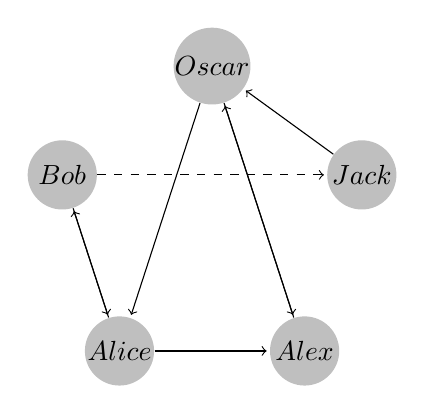
\begin{tikzpicture}[shorten >=1pt,->]
			\tikzstyle{vertex}=[circle,fill=black!25,minimum size=25pt,inner sep=0pt]

			\foreach \name/\angle/\text in {P-1/234/Alice, P-2/162/Bob, 
                                  P-3/90/Oscar, P-4/18/Jack, P-5/-54/Alex}
				\node[vertex,xshift=6cm,yshift=.5cm] (\name) at (\angle:2cm) {$\text$};
    
			\draw (P-1) -- (P-5);
			\draw[dashed,->] (P-2) -- (P-4);
			\draw (P-4) -- (P-3);
			\draw (P-3) -- (P-1);
			\draw (P-1) -- (P-2);
			\draw (P-2) -- (P-1);
			\draw (P-3) -- (P-5);
			\draw (P-5) -- (P-3);
  
		\end{tikzpicture}
		\caption{Communities of trust: Jack introduces Oscar to Bob's public-key certificate before Bob receives it.}
		\label{fig:web-of-trust}
	\end{center}
\end{figure}

Thus, we can figure out that PGP breaks the traditional hierarchical trust architecture with this \textit{web-of-trust} approach.\\

Let's get an example\footnote{Example from ''The PGP trust model''\cite{caronni2000}}: Bob want to exchange datas with Oscar, which he didn't knew before. But Jack, a colleague of Bob's, signs Oscar's public-key certificate whch he knows is authentic.\\
Oscar then forwards his signed certificate to Bob who wishes to communicate with Oscar privately.\\
Bob, who knows and truts Jack as an \textit{introducer}, find out, after verification, that Jack is among Oscar's certificate signer. Therefor, Bob can be confident that Oscar's public key is authentic.

However, had Bob not known or trusted Oscar's signers, including Jack, he would have been skeptical about the authenticity of Oscar's public-key. Oscar would have to find another introducer whom Bob trusts to sign Oscar's public-key certificate. This is illustrated in Figure \ref{fig:web-of-trust}.\\
This is illustrated in Figure 1, where the dotted arrow indicates ''Bob trusts Jack as introducer'' and the solid arrow indicates ''Jack trusts Oscar’s public key validity''. 


PGP also includes a public-key certificate and an introducer trustwhorthiness. They have different levels, for a public-key certificate they are:
\begin{itemize}
	\item \textit{Undefined:} we cannot say wether this public-key is valid or not.
	\item \textit{Marginal:} this public-key \textit{may} be valid but we cannot be sure.
	\item \textit{Complete:} we can be fully confident that this public-key is valid.
\end{itemize}
For an introducer, those levels of trustworthiness are the following:
\begin{itemize}
	\item \textit{Full:} this public-key is fully trusted to introduce another public-key.
	\item \textit{Marginal:} this public-key can be trusted to introduce another public-key, but, it is uncertain whether it is fully competent to do that.
	\item \textit{Untrustworthy:} this public-key should not be trustedto introduce another, therefore any occurence of this key as a signature on another public-key should be ignored.
\end{itemize}

Only the trustworthiness of public-key's validity is automatically evaluated by PGP. Introducer's worthiness is manually assigned by each user of to the public key, and exists only within each individual user's public-key ring\footnote{PGP allows users to have files representing multipke \textit{key rings} to store public or secret keys\cite{caronni2000}.}.

The big point is the use of such a tool in a world wide range: that is raisonnably not possible. We can assume to use it in a little group, where trustworthiness is effective, but in a more wide area, it is problematic to trust such a amount of people, or find trusted introducers. Furthermore, in a commercial use, there is no entity responsible when something goes wrong.


\subsection{SKIP (Simple Key-Management for Internet Protocol)}
\label{skip}

SKIP implements a linked-chain of two-sided node authenticators, where each node derives its informations from a sort of \textit{directory service}.\\
The problem is that SKIP happens at a low level, so it is transparent to the user; also assuming that the user has no control over security or other certification choices. So it has to be complemented by a second higher level protocol. Furthermore, SKIP does not support IP translation (such as NAT behind a firewall), that makes it quite useless.\\
So that protocol imediatly looks unapropriate for our study. In other way, SKIP does not exist anymore, so it is pointless to go further in it study.


\subsection{Thoughts about X.509, CAs and PGP}
\label{thoughts_old}

To be used in a commercial way (for responsabilities purpose), X.509, CAs and PGP need a centralized certification control system. However, there is a struggle between this need of centralization and the internet architecture (that is decentralized). This show us the uselessness of centralized governement controls, since we have no central government on the internet which give a world governance.\\
So the question emerging in there is: how can we (and do we need to) have a main control on an internet environement, to assure the goodness of datas and legitimacy of interlocutors?\\
Some answers have been made since then (thus since the publication of the original article), answers that we are going to explain further.


\subsection{DANE (DNS-Based Authentication of Named Entities)}
\label{dane}

DANE is not implemented yet, but a IETF team is working on the standard.\\
It has begin with a simple assert: why use a new trust infrastructure if we already have to use DNS to resolve a domain name?\\
From here, DNS must be securised, knowing that it is easily to set a MITM with DNS cache poisoning \cite{aa04} using the Kaminsky attack \cite{bor08}. That is the main purpose of DNSSEC: secure DNS. DANE allow to store keys in DNS. Thereby, \verb$www.example.org$ would be able to secure \verb$https://www.example.org$ without using a suspicious third part, just by putting its keys in the domain name that it controls. By its arborescent nature, \verb$example.org$ shall not be able to cheat on \verb$example.com$.\\

Lets give us an example:\\
From the classic schem, we have \textit{Alice}, the subscriber (\verb$alice.example.com$), \textit{Bob} its client, and \textit{Charlie}, the serious AC. There are three different scenarios:
\begin{itemize}
	\item \textit{Type 0:} Alice has got a certificate delivered by Charlie and is really satisfied by it. But Alice is afraid that \textit{Oscar} (a bad AC) forge a false certificate for its website. So Alice uses DANE to tell in DNS that Charlie and only Charlie is its AC.
	\item \textit{Type 1:} Alice has got a certificate delivered by Charlie, but fear that Charlie give its certificate to bad people. So Alice uses DANE to publish in DNS the origin of its certificate.
	\item \textit{Type 2:} that is the \textit{max scenario} in DANE. Alice doesn't trust ACs anymore, so it decides to emite it via DANE on DNS, that gives the entire responsability on DNS servers. 
\end{itemize}

This type is in a new register called TLSA\footnote{TLSA doesn't stand for anything: it is just the name of the RRtype (Record Resource type).} in DNS. Her is an example of a TLSA register:\\
\begin{Verbatim}[fontsize=\small]
_443._tcp.www.example.com. IN TLSA (
	0 0 1 d2abde240d7cd3ee6b4b28c54df0&34b9
	7983a1d16e8a410e4561cb106618e971 )
\end{Verbatim}
With:
\begin{itemize}
	\item \verb$443$ : the port used.
	\item \verb$tcp$ : the protocole used.
	\item \verb$www.example.com$ the domain name.
	\item \verb$0 x x$ : the type used, here it is a type 0 (\verb$1 x x$ for type 1 and \verb$2 x x$ for type 2).
	\item The rest is the certificate itself.
\end{itemize}

As we said before, DNS is not secured, so DNSEC has been deployed. DNSSEC is a protocol that allow to the DNS server (master) ti encrypt and sign its answer with a public key cryptographic system. It also permit to return a \verb$NXDOMAIN$ type (''No Such Domain'').\\
Nervertheless DNSSEC has some vulnaribilities such as:
\begin{itemize}
	\item Replay attacks
	\item Attacks against intermediaries: because of the hierarchic and centralized approch of DNS (there is only one root), the responsability of intermediaries is really high and a remote control by a thief should be bad (the thief controls the domain thus). History has proved that some of those intermediaries are not that trustworthy \cite{dan08} \cite{utk11}.
\end{itemize}

To make a conclusion about DANE, we have multiple points to point out:
\begin{itemize}
	\item Introducing a new register TLSA shall be very complicated, knowing that things are not moving that fast in DNS\footnote{Like it use to be with EDNS introduction few years ago.}.
	\item The validation necessity end to end is quite disturbing knowing that there is no standart and deployable solution for wide use  about the last kilometer securisation.
	\item DNSSEC is not possible behind a DNS proxy (which filter/break DNS answers to the point of creating a DoS for all TLS services.
\end{itemize}

Therefor, DANE is on a good way, particulary for communications between servers, where there is no (not much) constraints of security are (more) easily achievable. 

\subsection{Sovereign keys}
\label{sovkeys}



\subsection{CATA: Certificate Authority Transparency and Auditability}
\label{certtrans}

This protocol has been developped by a Google team few years ago \cite{LL11}. It is still in developpment \cite{certtransp2013} so it is not implemented and deployed yet. It also has to be improve, like everythign in computing sciences, in the early years.\\
CATA's purpose is a public list of all certificates that are emitted by CAs. Thus, clients are allowed to search in that public list, and verify that the received certificate is in that list, to be validate (if it is not in the list, it shall be rejected).\\
In that way, a(conscientious) domain administrator can have access to that list and monitor all fraudulent certificates for his domain.\\
For the moment, there are plenty of questions to answer like :
\begin{itemize}
	\item Who should hold those lists?
	\item How many lists should be created?
	\item How does the revokation should work?
	\item What should happen if a certificate is no longer available (path unreachable)?
\end{itemize}

\nocite{*}

\begin{thebibliography}{99}

\bibitem{gerck1998overview} E.Gerck, Overview of Certification Systems: X. 509, CA, PGP and SKIP, 1998.

\bibitem{skip1995} Ashar Aziz, Tom Markson, Hemma Prafullchandra, Sun Microsystems, Inc., v.06, 1995. https://tools.ietf.org/html/draft-ietf-ipsec-skip-06

\bibitem{skip2010user} Oracle, SunScreen SKIP User's Guide, Release 1.1, 2010. %http://docs.oracle.com/cd/E19957-01/805-5743/6j5dvnrfs/index.html

\bibitem{caronni2000} Caronni, G. (2000). Walking the web of trust. In Enabling Technologies: Infrastructure for Collaborative Enterprises, 2000.(WET ICE 2000). Proeedings. IEEE 9th International Workshops on (pp. 153-158). IEEE. %http://system.khl.mydns.jp/college/WOT/The_PGP_Trust_Model.pdf

\bibitem{bor08} Stéphane Bortzmeyer. Comment fonctionne la faille kaminsky ? http://www.bortzmeyer.org/comment-fonctionne-la-faille-kaminsky.html, 2008.

\bibitem{aa04} D. Atkins and R. Austein. Rfc 3833 : Threat analysis of the domain name system (dns). http://www.
ietf.org/rfc/rfc3833.txt, 2004.

\bibitem{dane2012} P Hoffman, J Schlyter, The DNS-based authentication of named entities (DANE) transport layer security (TLS) protocol: TLSA, 2012. https://www.rfc-editor.org/rfc/pdfrfc/rfc6698.txt.pdf

\bibitem{LL11} Ben Laurie and Adam Langley. Certificate authority transparency and auditability. http://www.links.
org/files/CertificateAuthorityTransparencyandAuditability.pdf, 2011.

\bibitem{certtransp2013} Laurie, B., Langley, A., \& Kasper, E. (2013). Certificate transparency (No. RFC 6962). %https://www.rfc-editor.org/rfc/pdfrfc/rfc6962.txt.pdf

\bibitem{rfc3647} Solo, D., Housley, R., \& Ford, W. (1999). Internet X. 509 public key infrastructure certificate and CRL profile. %http://tools.ietf.org/html/rfc2459

\bibitem{dan08} Dancho Danchev. Hackers hijack dns records of high profile new zealand sites. http://m.zdnet.com/blog/security/hackers-hijack-dns-records-of-high-profile-new-zealand-sites/3185, 2008.

\bibitem{utk11} Utkarsh. Domaining.com hacked. http://dotsutra.com/domain-names/industry-news/domaining-com-hacked/, 2011.

\end{thebibliography}

% Your document ends here!
\end{document}
